\documentclass[final,leqno,onefignum,onetabnum]{siamltexmm}
\usepackage{amsmath}
\usepackage{color,graphicx} 

\title{Detecting Hand movements from EEG Signals\thanks{Kaggle Grasp and lift competition. 
\url{https://www.kaggle.com/c/grasp-and-lift-eeg-detection}}} 

\author{Anirudhan J Rajagopalan, Michele Cer\'u\thanks{New York University (\email{ajr619@nyu.edu}; \email{mc3784@nyu.edu}). Questions, comments, or corrections to this document may be directed to this email address.}}

\begin{document}
\maketitle

\begin{abstract}
  This project aims to detect and classify the grasp and lift hand movements of a subject from EEG (Electroencephalography) recordings.
  Successful identification and classification of the recordings will help in developing Brain Computer Interfaces (BCI) that can be used to restore the ability of patients to do day-to-day tasks.
  We are provided with \~24 series of grasp and lift actions performed by twelve subjects.  We run our models using the first \~18 series as our training and the last \~2 series as our test set.
  We use the level1 predictions of the Kaggle contest winners as our baseline and try to compare the performance of our model against the level1 predictions of baseline.
  Using our simple pipeline we are able to show that we can get accuracy of 0.61 Mean Area Under the Curve (MAUC)\@.
\end{abstract}

\section{Introduction}

Electroencephalography (EEG) is used to record electrical activity of the brain.
It is typically noninvasive, with the electrodes placed along the scalp.  
In the Grasp And Lift (GAL) experiment twelve subjects were asked to perform lifting series in which the object's weight (165, 330, or 660g), surface friction (sandpaper, suede, or silk surface), or both, were changed unpredictably between trials, thus enforcing changes in fingertip force coordination.\cite{naturegal}
The hand movement of the subject was recorded by 3D sensors which were synchronized with the EEG cap thus providing us with the exact moment at which the GAL events happen.  With respecct to our goal of classifying the hand movements, we have to detect the following six events.

\begin{enumerate} 
  \item \textit{HandStart}: Beginning of the movement.
  \item \textit{FirstDigitTouch}: Making contact with the object.  
  \item \textit{BothStartLoadPhase}: Starting to load the object. 
  \item \textit{LiftOff}: Holding the object up.
  \item \textit{Replace}: Replacing the object in its original position.
  \item \textit{BothReleased}: Releasing the fingers from the object. 
\end{enumerate}

The EEG signals recorded by 32 electrodes fixed to the scalp are recorded at a frequency of 500Hz.  An added objective of this task is to make sure that we dont use any future data for doing predictions (No future data rule, as described in the data page of the challenge).  This restriction is imposed to mimic the real life scenarios in which such an application can be used, wherein, we will not have access to any of the future data while making predictions in real life.\cite{website:kaggle-competition}


This project aims to classify the hand movements of subjects by using EEG signal data.  We compare the performance of LinearSVM and GaussianSVM combined with VLAD and Bag of Features (BOF) feature representations.  We base our performance using the Area Under the Curve as described in the Kaggle challenge.  We try to reason the performance of our model with respect to the dataset by analysing the spatial relationship and variance of the features.  We then discuss about models that we might use to tackle this hard problem.

\section{Dataset Description}

\subsection{Sources and Format}
The dataset is provided by Kaggle Inc.\ for their Grasp and Lift Detection challenge\cite{website:kaggle-competition} sponsored by Way Consoritum\cite{website:way_consoritum}.  
The dataset consists of separate test and train zip files of size 153 MB and 915 MB respectively.  
The dataset expands to 447 MB and 3.1GB after extraction.  
Out of these datafiles, we cannot use the testset as they are being used for the competition submissions.  
The testset has only the *\_data.csv files with no corresponding *\_events.csv file.  
Since there is no *\_events.csv file we will not be able to learn or evaluate the performance of our models by using the test dataset provided in the challenge website.
So our effective usable dataset is only the training data which we partition into train and test set for training our models.

The dataset consists of two types of files: 
\begin{enumerate}
  \item{data.csv} --- CSV of series labels and values from the 32 electrode signals.
  \item{event.csv} --- CSV of series labels and event values.
\end{enumerate}
The sample dataset is included below for reference.

\begin{figure}[ht!]
  \centering
  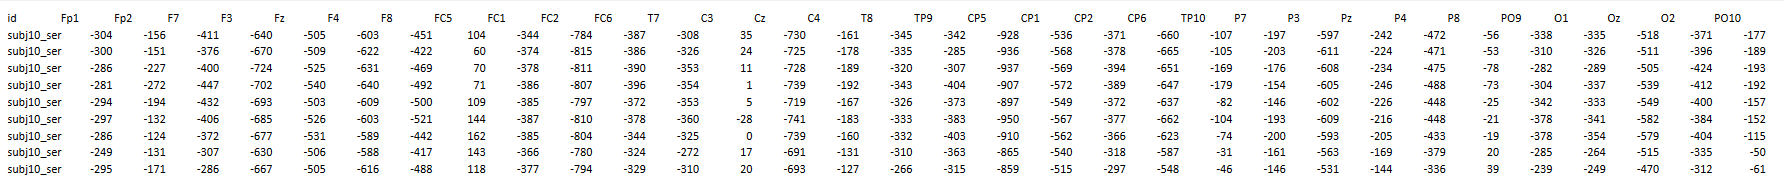
\includegraphics[width=1\textwidth]{images/sample_data}
  \caption{Sample Data format\label{fig:Sample_data}}
\end{figure}

\begin{figure}[ht!]
  \centering
  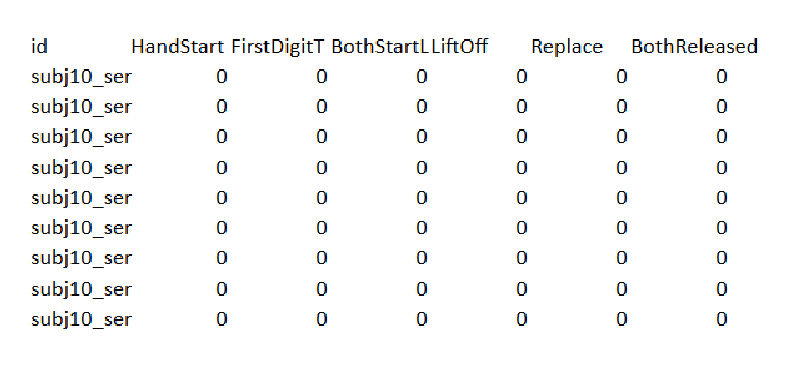
\includegraphics[width=0.5\textwidth]{images/sample_events}
  \caption{Sample Event format\label{fig:sample_events}}
\end{figure}

The event dataset will have a value of 1 corresponding to the event (stimulus) that is being performed at the instant of sampling.  There can be situations where there are multiple stimulus being triggered for the same EEG signal.  The objective is to classify (or) label the input EEG signals to the corresponding stimulus.

The total number of samples across the complete dataset is 17985850.

\subsection{Multilabeling or Multiclass classification}
The dataset can have multiple stimulus at the same time as shown in figure~\ref{fig:label_or_class}.
This is an important feature to consider as it forms the distinction between multiclass and multilabel classification problem.
\begin{figure}[ht!]
  \centering
  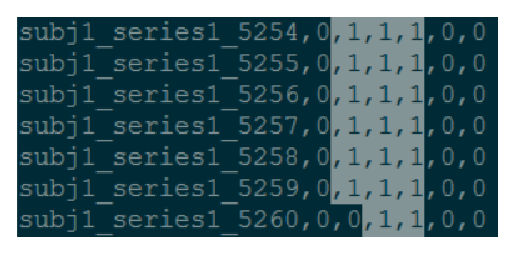
\includegraphics[width=0.5\textwidth]{images/multilabels}
  \caption{Multilabel or Multiclass classification problem.\label{fig:label_or_class}}
\end{figure}

\section{Problem Statement}
As described in the previous section, the objective is to classify/label the input EEG signals with their correspoinding stimulus.  
This is an inherently multilabel classification problem.  
We can reduce this to multiclass classification problem by considering the fact that the events happen in sequence.  
For example, BothReleased event is always followed by Replace which is always followed by LiftOff and so on and so forth.
Thus the problem of finding all events corresponding to the EEG signal can be decomposed into the problem of finding the start of the occurance of a particular event.

The constraint defined above simplifies our problem into a multiclass classification problem.  With proper feature selection and model selection we should be able to solve the problem effectively.

\section{Baseline}
\subsection{Choosing a baseline}
We considered the models (Cat and Dog solution) developed by Alexandre Barachant (a.k.a cat) and Rafal Cycon (a.k.a dog) for our baseline model.  
The solution by Cat and Dog won the first prize in the challenge and it makes logical sense to use that as our baseline.   
The cat and dog solution has three levels of models.
The first level of models use 
\begin{enumerate}
\end{enumerate}

\newpage

\bibliographystyle{siam}
\bibliography{references}

\end{document}
